\documentclass[tikz]{standalone}

\usepackage[utf8]{inputenc}
\usepackage[T1]{fontenc}
\usepackage{cmap}
\usepackage{amsmath}
\usepackage{amssymb}
\usepackage{verbatim}
\usepackage{bm}
\usepackage{siunitx}

\renewcommand{\familydefault}{\sfdefault}
\usepackage[cm]{sfmath}

\usepackage{tikz}
\usetikzlibrary{math}
\usetikzlibrary{bending}
\usetikzlibrary{decorations.pathreplacing}
\usetikzlibrary{decorations.pathmorphing}
\usetikzlibrary{fadings}
\usetikzlibrary{positioning}
\definecolor{cblue}{rgb}{0.396, 0.643, 0.82}
\definecolor{corange}{rgb}{1.0, 0.69, 0.416}
\definecolor{cgreen}{rgb}{0.471, 0.824, 0.471}
\definecolor{cred}{rgb}{1.0, 0.502, 0.502}
\definecolor{cpurple}{rgb}{0.863, 0.78, 0.937}

\def\symbhwaas{N_a}
\def\symbsteplen{\Delta d}
\def\symbsweeprate{f_s}
\def\symbsweepperiod{T_s}
\def\symbsweepdur{\tau_s}
\def\symbframerate{f_f}
\def\symbframeperiod{T_f}
\def\symbframedur{\tau_f}
\def\symbprf{f_\text{p}}
\def\symbspf{N_s}
\def\symbstartpoint{d_1}
\def\symbnumpoints{N_d}
\def\symbmur{r_\text{u}}
\def\symbcid{r_\ell}
\def\symbminmd{r_\text{min}}
\def\symbmaxmd{r_\text{max}}
\def\symbdcrnear{r_\text{near}}
\def\symbdcrfar{r_\text{far}}

\begin{document}

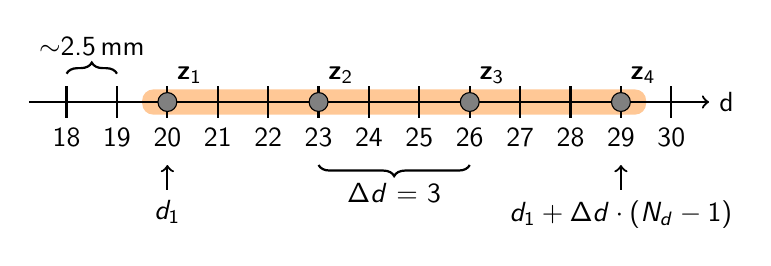
\begin{tikzpicture}[scale=0.8]
  \tikzmath{
    \dg = 0.8;
    %
    \nump = 4;
    \startp = 20;
    \steplen = 3;
    int \endp;
    \endp = \startp + (\nump-1)*\steplen;
    %
    \pad = 1.75;
    int \startpm;
    \endpp = \endp + 1;
    \startpm = \startp - 2;
    \endppp = \endp + \pad;
  }

  \fill [fill=corange, opacity=0.7, rounded corners] ({(\startp-0.5)*\dg}, -0.2) rectangle ({(\endp+0.5)*\dg}, 0.2);

  % axis
  \draw [thick, ->] ({(\startp-1-\pad)*\dg}, 0) -- (\endppp*\dg, 0) node[right]{d};
  % ticks
  \foreach \i in {\startpm, ..., \endpp}
    \draw [thick] ({\i*\dg}, 0) ++(0, 0.25) -- ++(0, -0.5) node[below]{$\i$};
  % measured points
  \foreach \i in {1, ..., \nump}
    \draw [fill=gray] ({(\startp+(\i-1)*\steplen)*\dg}, 0) circle (1.5mm) node[above right=3pt and 0pt]{$\bm{z}_{\i}$};
  % brace showing ~ 2.5 mm
  \draw [thick, decoration={brace, amplitude=4pt}, decorate] ({(\startp-2)*\dg}, 0.45) -- node[above=3pt] {\SI{\sim2.5}{mm}} ++(\dg, 0);
  % brace showing step
  \draw [thick, decoration={brace, amplitude=4pt}, decorate] ({(\startp+\steplen*2)*\dg}, -1) -- node[below=3pt]{$\symbsteplen$ = \steplen} ++(-\steplen*\dg, 0);
  % arrow showing start
  \draw [<-, thick] (\dg*\startp, -1) to ++(0, -0.4) node [below] {$\symbstartpoint$};
  % arrow showing end
  \draw [<-, thick] (\dg*\endp, -1) to ++(0, -0.4) node [below] {$\symbstartpoint + \symbsteplen \cdot (\symbnumpoints - 1)$};
\end{tikzpicture}

\end{document}
